\documentclass[12pt,openright,twoside,openany]{report}
\usepackage[a4paper,top=10mm,bottom=20mm,right=20mm,left=20mm]{geometry}
\usepackage[T1]{fontenc}
\usepackage[utf8]{inputenc}
\usepackage[swedish,british,french]{babel}
\usepackage{amsmath}
\usepackage{amssymb}
\usepackage{algorithm}
\usepackage{algpseudocode}
\usepackage{graphicx}
\usepackage{pict2e}
\usepackage{tabu}
\usepackage{booktabs}
\usepackage{bookmark,hyperref}
\usepackage{gensymb}
\usepackage{fancyhdr}
\usepackage{enumitem}
\graphicspath{{Figures/}}
\usepackage{pdfpages}




%Formatering av rubriker
%%%%%%%%%%%%%%%%%%%%%%%%%%%%%%%%%%%%%%%%%%%%%%%%%%%%%%%%%%%%%%%%%%%%%%%%%%%%%%%%%%%%%%%
\usepackage{titlesec, blindtext, color}
\titleformat{\chapter}[hang]{\Huge\bfseries}{\thechapter}{20pt}{}{}
\titlespacing*{\chapter}{0pt}{*0}{*0}
\titlespacing*{\section}{0pt}{*0}{*0}
\titlespacing*{\subsection}{0pt}{*0}{*0}
\titlespacing*{\subsubsection}{0pt}{*0}{*0}





%%%%%%%%%%%%%%%%%%%%%%%%%%%%%%%%%%%%%%%%%%%%%%%%%%%%%%%%%%%%%%%%%%%%%%%%%%%%%%%%%%%%%%%
\renewcommand{\listalgorithmname}{Liste des algorithmes}
\floatname{algorithm}{Algorithme}
\renewcommand{\algorithmicreturn}{\textbf{Renvoyer}}
\renewcommand{\algorithmicprocedure}{\textbf{procédure}}
\renewcommand{\Not}{\textbf{non}}
\renewcommand{\algorithmicendif}{\textbf{Fin Si}\ }
\renewcommand{\algorithmicendfor}{\textbf{Fin Pour}\ }
\renewcommand{\And}{\textbf{et}\ }
\renewcommand{\Or}{\textbf{ou}\ }
\renewcommand{\algorithmicrequire}{\textbf{Entrée:}}
\renewcommand{\algorithmicensure}{\textbf{Sortie:}}
%\renewcommand{\algorithmiccomment}[1]{\{#1\}}
\renewcommand{\algorithmicend}{\textbf{Fin}}
\renewcommand{\algorithmicfunction}{\textbf{fonction}}
\renewcommand{\algorithmicif}{\textbf{Si}}
\renewcommand{\algorithmicthen}{\textbf{alors}}
\renewcommand{\algorithmicelse}{\textbf{Sinon}}
\renewcommand{\algorithmicfor}{\textbf{Pour}}
\renewcommand{\algorithmicforall}{\textbf{Pour tout}}
\renewcommand{\algorithmicdo}{\textbf{faire}}
\renewcommand{\algorithmicwhile}{\textbf{Tant que}}
\newcommand{\algorithmicelsif}{\algorithmicelse\ \algorithmicif}
\newcommand{\algorithmicendif}{\algorithmicend\ \algorithmicif}
\newcommand{\algorithmicendfor}{\algorithmicend\ \algorithmicfor}


\def\frenchcontentsname{Sommaire}

%%%%%%%%%%%%%%%%%%%%%%%%%%%%%%%%%%%%%%%%%%%%%%%%%%%%%%%%%%%%%%%%%%%%%%%%%%%%%%%%%%%%%%%
\usepackage{tocloft} %Control the ToC formatting

\setlength{\parindent}{0pt}
\setlength{\parskip}{1em}
%\usepackage[a4paper,top=10mm,bottom=20mm,right=20mm,left=20mm,bindingoffset=6mm]{geometry}

%Formatting of page numbering (Comment to have the number centered)
%%%%%%%%%%%%%%%%%%%%%%%%%%%%%%%%%%%%%%%%%%%%%%%%%%%%%%%%%%%%%%%%%%%%%%%%%%%%%%%%%%%%%%%
\usepackage{fancyhdr}
\pagestyle{fancyplain}%
\fancyhf{} % clear all header and footer fields
\fancyfoot[RO,LE]{\thepage}
\renewcommand{\headrulewidth}{0pt}
%%%%%%%%%%%%%%%%%%%%%%%%%%%%%%%%%%%%%%%%%%%%%%%%%%%%%%%%%%%%%%%%%%%%%%%%%%%%%%%%%%%%%%%

\usepackage[hang, font=small, labelfont=bf]{caption}
\usepackage{subcaption}
\captionsetup{justification   = raggedright,
              singlelinecheck = false,
              format = hang}

\usepackage[
  backend=bibtex,
  %%%%% For NameYear citation
  %   style=authoryear,
  %   citestyle=authoryear-comp,
  %   sorting=nyt
  %%%%%
  %%%%% For Number citation
  style=numeric,
  citestyle=numeric,
  sorting=none,
  %%%%%
  maxcitenames=2,maxbibnames=99,
  natbib]
{biblatex}
\addbibresource{References.bib}



%%%%%%%%%%%%%%%%%%%%%%%%%%%%%%%%%%%%%%%%%%%
% DO NOT NEED TO CHANGE BEFORE THIS POINT %
%%%%%%%%%%%%%%%%%%%%%%%%%%%%%%%%%%%%%%%%%%%

\hypersetup{
    colorlinks=true,
    linkcolor=black,
    anchorcolor=black,
    citecolor=black,
    urlcolor=black,
    pdftitle={TITLE},  % Write your title here
    pdfauthor={Author Name}, % Write your name here
    }

\title{
	{\LARGE \textbf{ Génération aléatoire de nombres premiers} }\\ % Write your title here
    {\large Rapport L3 }\\
    {\large Projet Tutoré}\\
    {\vspace{10mm}}
    {
\includegraphics[width=0.6\textwidth]{télécharger.png}}
    }
\author{\textbf{Professeur accompagnant:} M. Castagnos\\\textbf{Ouvrage rédigé par:} \\Anass Bousseaden, Alexandre Bousquet et Baptiste Bédouret} %https://www.overleaf.com/project/60377afdf00e438677d1e0e3 Write your name here
\date{\today}





\begin{document}

\maketitle

\clearpage
\tableofcontents

\clearpage







\begin{center}
    \Huge \underline{\textbf{Sujet}}
\end{center}
Certains algorithmes de chiffrements à clef publique, comme le système RSA utilisent de grands nombres premiers. Nous verrons dans le cours d’arithmétique et cryptographie un test efficace permettant de savoir avec une grande certitude si un grand nombre est premier ou non. Cependant pour générer un grand nombre premier aléatoire ce test doit être appliqué un grand nombre de fois surtout si le nombre premier cherché doit avoir des propriétés particulières. Ceci rend la méthode coûteuse en temps et aussi en quantité d’aléas nécessaire. \\ \\
Il existe de nombreuses solutions visant à diminuer ce temps de calcul quitte à sacrifier un peu le caractère aléatoire des nombres premiers générés. D’autres solutions visent à produire des nombres premiers de manière proche de l’uniforme en diminuant la quantité d’aléas nécessaire.\\ \\
L’objectif du projet sera de comprendre et d’implémenter certaines de ces méthodes et de comparer les différents résultats expérimentaux vis à vis du temps de calcul, de la quantité d’aléas et du caractère aléatoire de la sortie.


\chapter{Introduction}

La cryptographie est l’ensemble de méthodes visant à sécuriser l’information et les communications numériques contre des adversaires. Elle utilise un système de chiffrement qui consiste à traduire un message donné en langage codé et un système de déchiffrement qui consiste à reconstituer le message initial à partir d'un message codé lorsqu'on connaît le code. 
L’utilisation des nombres premiers en cryptographie se base sur le système RSA qui est un système de chiffrement à clé publique. Cet algorithme a été décrit en 1977 par Ronald Rivest, Adi Shamir et Leonard Adleman. Le système RSA est original en ce sens que l'algorithme de chiffrement et la clé sont connus de tous, et cependant une seule personne peut déchiffrer le message.

\section{Fonctionnement de base du système RSA}

Les clés utilisées en cryptographie à clé publique sont en général construites à partir de grands nombres premiers choisis aléatoirement.
Un nombre premier $p$ est un entier strictement supérieur à 1, qui admet exactement deux diviseurs distincts, 1 et lui-même soit $p$.
Le système RSA utilise une paire de clés (des nombres entiers) composée d'une clé publique pour chiffrer et d'une clé privée pour déchiffrer des données confidentielles. Les deux clés sont créées par une personne, souvent nommée par convention Alice, qui souhaite que lui soient envoyées des données confidentielles. Alice rend la clé publique accessible. Cette clé est utilisée par ses correspondants (Bob, etc.) pour chiffrer les données qui lui sont envoyées. La clé privée est quant à elle réservée à Alice, et lui permet de déchiffrer ces données. La clé privée peut aussi être utilisée par Alice pour signer une donnée qu'elle envoie.

RSA est considéré comme un système de “sécurité absolue” pourvu qu’on utilise des grands nombres premiers.
Ainsi pour générer ces nombres premiers, on va tout d’abord dans un premier temps vérifier la primalité de ces nombres et ensuite dans un second temps on va parler des méthodes qui permettent de générer ces entiers, en utilisant des algorithmes de génération aléatoires de nombres premiers.

\section{Génération aléatoire de nombres premiers}

Notre objet de réflexion repose sur cet enjeu de générer de très grands nombres premiers de 1024 bits aléatoires que l'on ne puisse pas retrouver facilement. Nous voulons donc savoir avec une grande certitude si un grand nombre est premier ou non. Cependant pour générer un grand nombre premier aléatoire des tests doivent être appliqués un grand nombre de fois surtout si le nombre premier cherché doit avoir des propriétés particulières.\\
Ceci rend la méthode coûteuse en temps et aussi en quantité d’aléas nécessaire. C'est un gros défi car il n'est pas si simple de prouver qu'un nombre aussi grand soit premier en très peu de temps. On veut des algorithmes capable de donner une réponse quasi immédiate. Nous allons donc utiliser des théorèmes(Fermat, Miller-Rabin,...) et des factorisations d'entiers lorsque l'on reconnaît ou connaît sa forme (nombres de Mersennes, Sophie Germain). Notre étude se portera beaucoup plus sur la partie implémentation et l'étude expérimentale de ces algorithmes.
\\ 
\clearpage
Notre but final est de générer de très grands nombres premiers aléatoires afin d'avoir un système RSA infaillible. Nous allons donc découvir plusieurs tests rassemblant divers aléas en quantité plus ou moins grande.
Il existe de nombreux tests visant à diminuer le temps de calcul quitte à sacrifier un peu le caractère aléatoire des nombres premiers générés. D’autres test visent à produire des nombres premiers de manière proche de l’uniforme en diminuant la quantité d’aléas nécessaire.

D'une part, nous nous concentrerons sur deux grands axes qui sont les tests probabilistes de primalité et les tests de primalité.\\
D'autre part, nous aborderons la génération aléatoire de nombre premiers.

Nous n'aborderons pas le côté implémentation de nos algorithmes dans la section \ref{Test probabiliste de primalité} car les algorithmes ne sont pas trop "coûteux" ni difficile et nous ne trouvons donc pas nécessaire de développer une partie sur cet aspect. Nous exprimerons nos résultats expérimentaux qu'à partir de la section \ref{Test de primalité}.
\clearpage
\chapter{Test probabiliste de primalité}
\label{Test probabiliste de primalité}

Tout d'abord un algorithme probabiliste est un algorithme utilisant une source de hasard. Ces algorithmes sont rapides à l'exécution mais ils ne donnent pas toujours un résultat correct avec certitude.\\ Ils renvoient deux choses pour un $n$ fixé :\\
-Soit le test retourne que $n$ est \textbf{premier} et dans ce cas le résultat n'est pas certain.\\
-Soit le test retourne que $n$ est \textbf{composé} et dans ce cas on est certain.\\
Ainsi un test probabiliste nous donne avec certitude que $n$ est composé.
Mais on ne peut jamais être sûr que $n$ est premier.


Il y a plusieurs familles de tests probabilistes. 
Les trois grands tests connus sont le test de Fermat, le test de Solovay-Strassen et le test de Miller-Rabin.
Le test de Miller-Rabin est analogue au test de primalité de Solovay-Strassen, que l'on ne traitera pas, mais cependant toujours plus efficace que ce dernier et le test de Fermat.

On s'accordera à dire en pratique qu'il faut que l'algorithme est une probabilité inférieure à $\left(\frac{1}{2}\right)^{80}$ d'échouer. Il faut alors s'assurer que le paramètre de sécurité garantit un tel niveau de sécurité pour une taille de bits donnée.

On se concentrera dans cette deuxième partie sur le test de Fermat et de Miller-Rabin. 


\section{Test Probabiliste Première Idée}
Avant toute chose, si on pense à un test probabiliste de primalité la chose la plus simple à laquelle on pense est le théorème de Fermat ou alors de chercher un diviseur du nombre compris entre 2 et sa racine.\\
Ainsi, une première idée pour établir un test de primalité on se base
sur le petit théorème de Fermat que l'on implémente de la manière suivante. \\
Pour dire si $n$ est premier ou pas on calcule  $ b = a^{n-1} \mod n$.\\ On observe ainsi que : \\  
- Si  $ b \not \equiv 1 \mod n$ alors on est sur que $n$ est composé.\\
- Si $ b \equiv 1 \mod n$ alors $n$ est peut-être premier. On teste avec un autre $a$ pour vérifier si $n$ est premier.\\
\\
Évidemment on voit que cet algorithme n'est qu'une idée générale mais pas applicable en réalité car pas assez fort et utile pour vérifier la primalité d'un nombre. Il permet donc d'introduire le test de Fermat qui suit.

\section{Test de Fermat}
En algorithmique, le test de primalité de Fermat est un test de primalité probabiliste basé sur le petit théorème de Fermat. 
Il est de type Monte-Carlo. Cette spécificité nous permet de savoir à coup sûr que le nombre est composé.
Cependant, il peut se tromper s'il prétend que le nombre est premier. On va voir quels sont les nombres qui font échouer ce test et donc ce théorème.
\clearpage
\subsection{Théorème de Fermat} 

\underline{\textbf{Théorème :}}\textit{(Petit Théorème de Fermat)}
\begin{center}
    Soit $p$ un nombre premier et soit $a$ non divisible par $p$ alors $a^{p-1} \equiv 1 \mod p$.
\end{center}
La réciproque du théorème est vraie en effet si $p$ est composé on prend un diviseur non trivial de $p$ nommé $d$. Pour $1<d<p$ on a  $d^{\ p-1} \not \equiv 1 \mod p$.\\
Par contre, si on fixe la base $a$, il se peut que $a^{p-1}\equiv 1\mod p$ sans que $p$ ne soit premier. Ce sont des nombres pseudos-premiers dont on verra la définition.\\

\underline{\textbf{Théorème :}}\textit{(variante)}

\begin{center}
    Pour tout $a \in \mathbb{Z} $ et $p$ premier, $a^{p} \equiv a \mod p$.
\end{center}
Néanmoins ici la réciproque du théorème est fausse. Ce sont les nombres pseudo-premiers qui pour toutes les valeurs de $a$ qui sont premières avec $p$ ,autrement appelé nombre de Carmichael, font échouer cette réciproque. Ainsi, le petit théorème de Fermat donne une condition nécessaire pour qu'un nombre $p$ soit premier mais non suffisante. 
\subsection{Le test de Fermat} 
Ce premier algorithme permet de vérifier le petit Théorème de Fermat.\\
Il permet de comprendre l'idée utilisée pour construire le test de Fermat.
\begin{algorithm}[h!]
\caption{Fermat($n$)}
\begin{algorithmic}[1]
\Require{$n$ un entier} \Comment{Petit théorème de Fermat}
\Ensure{$n$ est premier ou composé}
\State Choisir $a$ un entier tel que $2\leq a \leq n-1$
\If{$a^{n-1} \equiv 1 \mod n$} \Return "premier"
\EndIf
\State \Return "composé"
\end{algorithmic}
\end{algorithm}

Ce deuxième algorithme est le test de Fermat. Il itère $t$ fois en utilisant le théorème de Fermat afin de vérifier si $n$ est premier. On sait que s'il retourne "composé" alors $n$ est composé mais s'il retourne "premier" on sait que $n$ n'est pas forcément premier.
\begin{algorithm}
\caption{TestFermat($n$,$t$)}
\begin{algorithmic}[1]
\Require{$n\geq 3$ impair et $t$ un paramètre de sécurité}
\Ensure{$n$ est premier ou composé}
\For{$i$ \textbf{allant de} 1 \textbf{à} $t$}
\State Choisir $a$ un entier tel que $2\leq a \leq n-2$
\State Calculer  $r=a^{n-1} \mod n$
\If{$r \not = 1$} \Return "composé" 
\EndIf
\EndFor
\State \Return "premier"
\end{algorithmic}
\end{algorithm}

Soit $n\geq 3$ impair, la probabilité que TestFermat($n$,$t$) déclare que $n$ est “premier” est inférieure à $\left(\frac{1}{2}\right)^{t}$ car il échoue pour au moins la moitié des choix de $a \in \mathbb {Z} /n\mathbb {Z}$. \\ \\
\underline{\textbf{Preuve :}}\\
Considérons l'ensemble $H$ des valeurs de $a \in \mathbb {Z} /n\mathbb {Z}$ qui ne font pas échouer le test, ainsi $H= \{a \in \mathbb {Z} /n\mathbb {Z}  : a^{n-1} \equiv 1 \mod n \}$. On a alors $Card(H) < \varphi(n)$. $H$ est un sous-groupe strict du groupe multiplicatif 
$(\mathbb {Z} /n\mathbb {Z} )^{\times }$. Par le théorème de Lagrange, $Card(H)\leq {\dfrac {n-1}{2}}$. Ainsi, en itérant $t$ fois le test de Fermat de la façon suivante, la probabilité de retourner "premier" si $n$ est composé est plus petite que $\left(\frac{1}{2}\right)^{t}$.
\subsection{L'inconvénient}
Le désavantage de cet algorithme est bien sur le fait qu'il existe des nombres qui passent le test alors qu'ils ne sont pas "premier".
\\ \\
\underline{\textbf{Proposition :}}
On dit qu’un nombre $n$ est pseudo-premier en base $a$ si $n$ n’est pas premier et vérifie l’égalité $a^{n-1} \equiv 1 \mod n $.

\underline{\textbf{Proposition :}} Soit un nombre Carmichael $n$ est un entier composé tel que $a^{n-1} \equiv 1 \mod n$ pour tous les entiers $a$ qui satisfont $\text{pgcd}(a,n)=1$. C'est donc un nombre-pseudo premier avec un condition en plus qui est que $\text{pgcd}(a,n)=1$.

Finalement, les nombres pseudo-premiers et  de Carmichael font échouer à coup sûr le test de Fermat renvoyant "premier" alors qu'ils sont "composé" même si le paramètre $t$ d'itération est élevé. Nous savons que depuis 1994, il en existe une infinité. Or, cet algorithme ne sera pas utilisé en pratique pour trouver si un nombre est premier car il y a trop de nombres pseudo-premiers qui font échouer le test mais il permet d'avoir une approche en terme de test sur les nombres premiers.
Cette carence dans le test de Fermat est éliminée dans les tests probabilistes de primalité de Solovay-Strassen et Miller-Rabin en s’appuyant sur des critères qui sont plus forts que le théorème de Fermat.


\section{Test de Miller-Rabin}

 On le considère comme l'algorithme le plus efficace pour les test probabilistes et ce test est une amélioration du test de Fermat. Il est beaucoup moins évident que Fermat mais meilleur car il s'appuie sur des critères plus fort qui ne font pas échouer l'algorithme pour les nombres de Carmichael. La probabilité donc pour cet algorithme de se tromper est beaucoup plus basse que pour les test de Fermat ce qui est un très gros atout. On verra dans la suite les avantages et la probabilité de cet algorithme de se tromper.\\
 Le test de Miller Rabin est un algorithme probabiliste très rapide. Il est très utilisé en cryptographie asymétrique notamment lors du chiffrement RSA pour engendrer les grands nombres premiers nécessaires.\\ Étant donné un nombre entier $n$, il retourne soit:

-\textbf{Composé}: dans ce cas on sait de façon certaine que $n$ est composé

-\textbf{Premier}: dans ce cas on sait que $n$ est probablement premier

Dans le cas "composé" on dispose de plus d’un " témoin " prouvant que $n$ est composé. Pour le cas "premier", par répétitions de l’algorithme, on peut rendre aussi faible que l’on veut la probabilité qu’un nombre composé $n$ soit déclaré probablement premier.
\clearpage

\subsection{Propositions et Théorème de Miller-Rabin} 

\underline{\textbf{Proposition :}} Soit $n$ un nombre premier impair que l’on décompose sous la forme $n= 2^s \times r +1$. Avec $s$ et $r$ deux entiers naturels tel que $s$ est non nul et $r$ impair. Soit $a \in \mathbb{N}$ tel que $pgcd(a,n)=1$, on a: 
\begin{enumerate}[label=\roman*)]
 \item  Soit  $a^r \equiv 1 \mod n$ ;
 \item  Soit $ a^{2^{i}\times r} \equiv -1 \mod n$ pour certains $i$ tels que $0\leq i \leq s-1$.
\end{enumerate}

Ainsi avec cette proposition on arrive à la définition suivante:\\ \\
\underline{\textbf{Définition :}}
Soit $n$ un nombre premier impair composé de la forme $n= 2^s\times r +1$. Avec $s$ et $r$ deux entiers naturels tel que $s$ est non nul et $r$ impair. Pour tout $a \in [1,n-1]$, on a: 
\begin{enumerate}[label=\roman*)]
 \item  Si $a^r \not\equiv 1 \mod n$ et $ a^{2^{i}\times r} \not\equiv -1 \mod n$, pour tout $i$ tel que $0\leq i \leq s-1$ , alors $a$ est un témoin pour $n$ ; 
 \item  Sinon si $a^r \equiv 1 \mod n$ ou $ a^{2^{i}\times r} \equiv -1 \mod n$, pour certains $i$ tels que $0\leq i \leq s-1$ alors $n$ est dit être un pseudo-premier fort en base $a$.
\end{enumerate}

\underline{\textbf{Théorème :}} Soit $n$ un entier impair composé $>$ 9, avec $n= 2^s\times r +1 $ pour $r$ impair. Alors il existe au plus $\dfrac{\varphi(n)}{4}$ menteurs forts $a$, pour $1<a<n$, c'est-à-dire des entiers $a$ vérifiant soit $a^r \equiv 1 \mod n$, soit $ a^{2^{i}\times r} \equiv -1 \mod n$, pour un certain $i$ tel que $0\leq i \leq s-1$.

Tout ceci nous conduit au test de Miller-Rabin.


\subsection{Le test de Miller-Rabin} 

Cet algorithme est le test de Miller-Rabin. Il itère $t$ fois afin de vérifier si $n$ est premier. Or le nombre $n$ peut être déclaré premier avec une faible probabilité d'erreur en ajustant le paramètre de sécurité $t$ pour que la probabilité d'échouer soit inférieure à $\left(\frac{1}{2}\right)^{80}$ .

\begin{algorithm}[h!]
\caption{MillerRabin($n$,$t$)}
\begin{algorithmic}[1]
\Require{$n\geq 3$ impair et $t$ un paramètre de sécurité}
\Ensure{$n$ est premier ou composé}
\State \textbf{Ecrire} $n= 2^s \times r +1 $ tel que r est premier
\For{$i$ \textbf{allant de} 1 \textbf{à} $t$}
\State Choisir $a$ un entier tel que $2\leq a \leq n-2$
\State Calculer  $y=a^{r} \mod n$
\If{$y \not = 1$ et $y \not = n-1$} faire 
\State i=1
\While{ $i \leq s-1$ et $y\ne n-1$}
\State Calculer $ y=y^2 \mod n$
\State \textbf{si} $y = 1$ \Return "composé"
\State $i=i+1$
\EndWhile
\State \textbf{si} $y\ne n-1$ \Return "composé"
\EndIf
\EndFor
\State \Return "premier"
\end{algorithmic}
\end{algorithm}

\clearpage
\underline{\textbf{On propose une preuve du théorème : }}

On écrit $ n = \prod_i p_i^\varepsilon^_i $ la décomposition unique de $n$ en facteur premiers, $n-1=2^\alpha m$ avec $m$ impair.

On pose $p_i-1 = 2^{\alpha_i}m_i$ avec $m_i$ impair.

Finalement notons $\beta = \min\{\alpha_i , p_i|n \}$ de sorte que $\beta$ soit 
la plus grande puissance de 2 divisant tout les $p_i-1$.

on considère les ensembles définit comme suit :
\begin{center}
    $N_+ = \{ x \in \mathbb{Z}/n\mathbb{Z} , x^{2^{\beta-1}m}={1}\}$ , $N_- = \{ x \in \mathbb{Z}/n\mathbb{Z} , x^{2^{\beta-1}m}={-1}\}$ , $N=N_+\cup N_-$
\end{center}
 
enfin $$M=\{x \in \mathbb{Z}/n\mathbb{Z}\; |\;  x^m=1 \text{ ou } x^{2^jm}=-1 \text{ pour }  j\in \{ 0,1,...,\alpha-1\} \} $$ 

On va montrer successivement que $M\subset N$, puis que $\#N=\frac{\varphi(n)}{4}$, ce qui permet de conclure.

Commençons par vérifier que $M\subset N$. Cela repose sur le théorème chinois qui nous permet de décomposer $\mathbb{Z}/n\mathbb{Z}^*$ en produit de groupe cyclique :

$$\mathbb{Z}/n\mathbb{Z}^*\simeq \prod_i \mathbb{Z}/p_i^{\varepsilon_i}\mathbb{Z}^* $$

On sait que chaque composante du produit de droite est de cardinal $p_i^{\varepsilon_i-1}(p_i-1)$.
Cela étant, pour $x\in \mathbb{Z}/n\mathbb{Z}^*$, si $x^m=1$, il est évident que $x \in N .$ Si maintenant $x^{2^j m}=-1$ pour un $j \in \{0, 1, . . . , \alpha - 1\}$,
alors $(x^m)^{2^j}=-1 \mod n$. A fortiori, $(x^m)^{2^j}=-1\mod p_i^{\varepsilon_i}$ pour tout i. En particulier, cela veut dire que $x^m$ est d'ordre $2^{j+1}$ modulo $p_i^{\varepsilon_i}$ pour tout i.

Par conséquent $2^{j+1}$ divise $\varphi(p_i^{\varepsilon_i})$ si bien que  $j+1<\beta$.

il en résulte bien que $x\in N$. 

- Dénombrer $N_+$ revient à compter les solutions de l'équation $x^{2^{\beta-1}m}=1 \mod p_i^{\varepsilon_i}$ pour tout i. On a donc :

$$\#N_+ = \prod_i \text{pgcd}\left( 2^{\beta -1 }m,p_i^{\varepsilon_i-1}(p_i-1) \right) =\prod_i 2^{\beta-1}\text{pgcd}(m,p_i-1)  $$

De la même façon, dénombrer $N_-$ revient, pour chaque diviseur premier $p_i$ de $n$, à compter le nombre  de solutions  de l'équation $x^{2^{\beta-1}m}=-1 \mod p_i^{\varepsilon_i}$. On remarque alors que :

$$\{x \in \mathbb{Z}/p_i^{\varepsilon_i}\mathbb{Z}\; ,x^{2^{\beta -1}m}=-1 \}=\{x \in \mathbb{Z}/p_i^{\varepsilon_i}\mathbb{Z}\; ,x^{2^{\beta}m}=1 \}\backslash \{x \in \mathbb{Z}/p_i^{\varepsilon_i}\mathbb{Z}\; ,x^{2^{\beta -1}m}=1 \}$$


si bien que :

\begin{align*}
    \{x \in \mathbb{Z}/p_i^{\varepsilon_i}\mathbb{Z}\; ,x^{2^{\beta -1}m}=-1 \}&=\text{pgcd}\left( 2^{\beta  }m,p_i^{\varepsilon_i-1}(p_i-1) \right)-\text{pgcd}\left( 2^{\beta -1 }m,p_i^{\varepsilon_i-1}(p_i-1) \right)\\
    &=2^{\beta}\text{pgcd}(m,p-1)-2^{\beta-1}\text{pgcd}(m,p-1)\\
    &=2^{\beta-1}\text{pgcd}(m,p-1)
\end{align*}

Ainsi $\#N_+=\#N_-$ et :

$$\#N=2\prod_{p|n} 2^{\beta -1}\text{pgcd}(m,p-1)$$

Il nous faut donc prouver que :

\begin{align}
    \dfrac{\#N}{\varphi(n)}=2\prod_{p|n}\dfrac{2^{\beta-1}\text{pgcd}(p-1,m)}{(p-1)p^{\varepsilon_p-1}} \overset{?}{\leq} \dfrac{1}{4} \Leftrightarrow \prod_{p|n}\dfrac{(p-1)}{2^{\beta-1}\text{pgcd}(p-1,m)} p^{\varepsilon-1} \overset{?}{\geq} 8 
\end{align}

Comme $\dfrac{(p-1)}{2^{\beta-1}\text{pgcd}(p-1,m)}$ est un entier supérieur a 1, si $n$ est divisible par au moins trois premiers distincts, l'inégalité (2.1) est satisfaite. Dans le cas ou $n$ ne possède que deux premiers $p$ et $q$ dans sa décomposition primaire, on distingue deux possibilités. Soit, par exemple $\varepsilon_p \geq 2 $ auquel cas le membre de gauche de (2.1) est clairement $\geq 4p \geq 8$.
Soit $n=pq$; le seul cas de figure ou l'inégalité (2) pourrait ne pas être satisfaite, c'est quand :

$$\dfrac{(p-1)}{2^{\beta-1}\text{pgcd}(p-1,m)}=\dfrac{q-1}{2^{\beta-1}\text{pgcd}(q-1,m)}=2$$

ou encore :
$$
\left\{
    \begin{array}{ll}
        p-1=2^{\beta}\text{pgcd}(p-1,m)=2^{\alpha_p m_p}
        \\
        q-1=2^{\beta}\text{pgcd}(q-1,m)=2^{\alpha_q m_q}
    \end{array}
\right.
$$

cela implique :

$$
\left\{
    \begin{array}{ll}
        \alpha_p=\alpha_q=\beta
        \\
        \text{pgcd}(p-1,m)=m_p
        \\
        \text{pgcd}(q-1,m)=m_q
    \end{array}
\right.
$$

Ainsi $m_p$ doit diviser $m$ et $(p-1)$. Ceci est impossible car en raisonnant modulo $m_p$ on s'aperçoit que :

$$2^{\beta}m_q=q-1\equiv pq-1\equiv n-1 \equiv 2^\alpham \equiv 0 \mod m_p \implies m_p|m_q$$.

Par symétrie, on a aussi $m_q|m_p$ donc $m_q=m_p$ puis $p=q$, ce qui est absurde. Enfin, si $n$ est la puissance d'un seul premier $n=p^{\varepsilon_p}$ alors, comme $n$ est supposé impair et plus grand que $9$, on a $p\geq 5$ et $\varepsilon_p \geq 2$ ou $p\geq 3$ et $\varepsilon_p \geq3$; dans les deux cas l'inégalité (2) est encore trivialement satisfaite.

\clearpage
\subsection{L'avantage}

Tout d'abord, le test de Miller-Rabin est très efficace. La probabilité qu'un $a$ pris au hasard soit un menteur fort est au plus $\frac{1}{4}$. Si on répète t fois l'algorithme la probabilité qu'un nombre composé impair de p bits (compris pris entre $2^p - 1$ et $m = 2^p$) soit déclaré probablement premier par l'algorithme de Miller-Rabin est inférieure à $\left(\frac{1}{4}\right)^{t}$.
L’algorithme arrive donc très rapidement à détecter un nombre composé avec une marge d’erreur très faible mais non nulle.

Un autre avantage est sa complexité. Dans le test de Miller-Rabin, on calcule tout d'abord au moyen de l'algorithme d'exponentiation modulaire rapide  $y$, tel que $y=a^{r} \mod n$. Le coût est  $O(log(r)*log^2(n))$. Puis on éléve au carré $y$ tel que $y= a^{2^{i}*r} \mod n $ pour tout $i$ dans $ \{1,...,s-1\} $. Son coût est en $O((log(n)^2)$. Enfin, on répete t fois l'algorithme est sa complexité devient $O(t*(log(n))^3)$. Ainsi ce test à un temps polynomial efficace.
\chapter{Test de primalité}
\label{Test de primalité}
Les tests de primalité sont des algorithmes permettant de déclarer et démontrer à coup sûr que le nombre est premier ou non sans utiliser d'aléatoire. Ces tests sont exercés sur des nombres entiers positifs qui peuvent être prouvés comme premiers. Ces algorithmes de primalité sont généralement plus coûteux sur le plan informatique que les tests probabilistes de primalité de la section \ref{Test probabiliste de primalité}. Ainsi, avant d’appliquer l’un de ces tests à un candidat primaire $n$, le candidat doit être soumis à un test de primalité probabiliste tel que Miller-Rabin pour améliorer le temps de calcul. Dans cette partie nous nous intéresserons à deux types de tests d'une part celui de Lucas-Lehmer qui teste les nombres de Mersenne et d'autre part celui de Pocklington qui prouve qu'un nombre est premier par la factorisation partielle $n-1$. Nous n'aborderons pas le test utilisant les courbes elliptiques car nous n'avons pas abordé cette notion.

\section{Test de Lucas-Lehmer}

Le test de Lucas-Lehmer est un algorithme efficace permettant de prouver et tester si un nombre de Mersenne est premier. Or c'est une classe de nombres avec une propriété particulière.
Ainsi pour cela rappelons la définition d'un nombre de Mersenne.

\subsection{Les nombres de Mersenne}

\underline{\textbf{Définition :}}
Soit  $p \geq 2$ un entier, un nombre de Mersenne est un entier de la forme $M_p=2^p -1$.\\
Si $M_p$ est premier alors il est appelé nombre premier de Mersenne.\\
\\
Evidemment tous les nombres de Mersenne ne sont pas premiers.
\subsection{Théoreme de Lucas-Lehmer}
Les conditions suivantes sont nécessaires et suffisantes pour qu’un nombre de Mersenne soit premier.

\underline{\textbf{Théorème :}}
Soit $p \geq 3$. Le nombre de Mersenne est premier si les deux conditions suivantes sont satisfaites:
\begin{enumerate}[label=\roman*)]
 \item $ p $ est premier ;
 \item  la suite d’entier définies par, $u_0=4$ et  $u_{i+1}=(u_i^2 -2)\mod n$ pour $i \geq 0$ satisfait $u_{p-2}=0 $;
\end{enumerate}

Ce théorème conduit au test de Lucas-Lehmer, un algorithme en temps polynomial permettant de déterminer avec certitude si un nombre de Mersenne est premier. 

\clearpage

\subsection{Le test de Lucas-Lehmer}

\begin{algorithm}
\caption{testLucasLehmer($p$)}
\begin{algorithmic}[1]
\Require{Un nombre de Mersenne $n=2^p-1$ avec $p\geq3$}
\Ensure{$n$ est premier ou composé}
\For{$i$ \textbf{allant de} 2 \textbf{à} $\left\lfloor\sqrt{p}\right\rfloor$}
\If{$i$ divise $p$} \Return "composé" 
\EndIf
\EndFor
\State Choisir $u=4$ 
\For{$i$ \textbf{allant de} 1 \textbf{à} $p-2$}
\State $u\leftarrow u^2-2 \mod n$
\EndFor
\If{$u = 0$} \Return "premier" 
\EndIf
\State \Return "composé"
\end{algorithmic}
\end{algorithm}
Cet algorithme sert à tester une classe de nombres premiers bien spécifiques mais il est le plus efficace si le nombre premier est un nombre premier de Mersenne. \\
\\ \underline{\textbf{Expériences :}}
L'algorithme nous donne des résultats presque immédiats ($\approx 3\, s.$) pour des nombres de 20000 bits ce qui montre son efficacité. Malheureusement, la première boucle "pour" nous ralentit considérablement pour un nombre $p\geq$ 500000 bits.

\section{Test de Pocklington}

Ce test permet de prouver qu'un nombre entier $n$ est premier, à condition que la factorisation partielle de $n-1$ soit connue. Ce n'est à priori pas évident d'envisager une méthode telle que la factorisation de $n-1$ soit un sous-problème. Parce que en terme de bits $n-1$ et $n$ sont presque égaux. Néanmoins, la factorisation de $n-1$ peut être plus facile à calculer si $n$ a une forme spéciale ou lorsque le $n$ candidat est construit par des méthodes spécifiques comme nous le verrons dans la section suivante. Le test de Pocklington n'est pas vraiment un test car il résulte du théorème de Pocklington mais il est nécessaire de comprendre le théorème et de l'implémenter car il sera utile pour la génération de nombres premiers.

\subsection{Théoreme de Pocklington}

\underline{\textbf{Proposition :}}
Soit un entier $n\geq3$. Alors $n$ est premier si et seulement si il existe un entier $a$ satisfaisant : 

\begin{enumerate}[label=\roman*)]
 \item $a^{n-1} \equiv 1 \mod n $ et
 \item  $a^{\frac{n-1}{q}} \not \equiv 1 \mod n$ pour tout diviseur premier $q$ de $n-1$
\end{enumerate}

Ce résultat vient du fait que $(\mathbb {Z} /n\mathbb {Z} )^{\times }$ a un élément $a$ d'ordre $n-1$ si et seulement si $n$ est premier. Donc cet élément $a$ vérifie i) et ii).\\ D'après cette proposition nous pourrions faire un test de primalité pour $n$. Pour tester si $n$ est premier, on choisit $a \in \mathbb{Z}/n\mathbb{Z}$ et on vérifie les hypothèses i) et ii) pour vérifier si $a$ est d'ordre $n-1$. On sait qu'il y a $\varphi(n-1)$ éléments d'ordre $n-1$ dans $ \mathbb{Z}/n\mathbb{Z}$. Ainsi, si $a$ n'est pas d'ordre $n-1$ on réitère avec un autre $a$ choisit. Mais pour cela il faut établir un nombre d'itération pour ne pas que le test soit trop "gourmand". Pour cela le bon nombre d'itération est de l'ordre de $\dfrac{n-1}{\varphi(n-1)}$ .\\ Enfin, si le test ne trouve pas de $a$ qui fonctionne après ce nombre d'itérations alors $n$ est probablement composé, il reste à vérifier si $n$ est composé en faisant le test de Miller-Rabin en parallèle afin d'être sûr.
\\ \\
Cette proposition et ce test nous amène a un théorème central permettant de prouver la primalité de $n$ en ne connaissant que la factorisation partielle de $n-1$.

\underline{\textbf{Théorème :}}
Soit $n \geq 3$ un entier, et $n=RF+1$.  F est produit de facteur premier c’est-à-dire $F=\prod\limits_{j=1}^t q_j^{\alpha_j}$. S'il existe un entier $a$ qui satisfait :

\begin{enumerate}[label=\roman*)]
 \item   Soit $a^n-1 \equiv 1 \mod n$ et
 \item   Soit $ \text{pgcd}(a^{n-1/q_j} -1,n)=1$ pour $j$, $1\leq j \leq t$.
\end{enumerate}

Alors chaque diviseur premier $p$ de $n$ est congru à $1 \mod F$. En particulier : si $F\geq \sqrt{n}-1$ alors $n$ est premier.

\underline{\textbf{Preuve :}}
 
\subsection{Le test de Pocklington}

\begin{algorithm}[h!]
\caption{testPocklington($n$,$L$)}
\begin{algorithmic}[1]
\Require{$n=RF+1$, $L$ la liste des facteurs premiers de $F$ }
\Ensure{$n$ est premier ou composé}
\State \textbf{Choisir} $a$ un entier tel que $2\leq a \leq n-2$
\If{$a^{n-1} \not \equiv 1 \mod n$} \Return "probablement composé" 
\EndIf
\For{\textbf{tout }$q$ dans $L$}
\State $R=a^{\frac{n-1}{q}} \mod n$
\If{$\text{pgcd}(R,n) \not = 1$} \Return " probablement composé" 
\EndIf
\EndFor
\State \Return "premier"
\end{algorithmic}
\end{algorithm}

Pour être plus précis on doit déterminer un nombre d'itérations afin d'avoir un algorithme optimal. Pour cela nous arrivons à une proposition nous permettant de calculer la probabilité de choisir une base $a$ qui convient pour i) et ii).

\underline{\textbf{Proposition :}}
Soit $n \geq 3$ un entier, et $n=RF+1$.  F est produit de facteur premier c’est-à-dire $F=\prod\limits_{j=1}^t q_j^{\alpha_j} > \sqrt{n}-1$  et $\text{pgcd}(R,F)=1$. Alors, la probabilité de choisir aléatoirement une base $a$ , $1\leq a \leq n-1$ satisfaisant: i) et ii) est $\prod\limits_{j=1}^t (1-\frac{1}{q_j}) \geq 1 - \sum\limits_{j=1}^{t} \frac{1}{q_j}  $.
\\
\underline{\textbf{Remarque :}}
Cette propostion nous amène au fait que le bon nombre d'itérations qui doit être fait est $T$ où $P^T \leq (\frac{1}{2})^{100}$ et $P=1-\prod\limits_{j=1}^t (1-\frac{1}{q_j})$. Nous avons eu du mal à bien calculer ce $T$ pour garantir cette sécurité demandée c'est pourquoi nous avons mis $T=1$ mais il faudrait adapter $P$ et $T$ à notre nombre de facteurs premiers de $F$.

\\
On a donc l'algorithme suivant pour le test de Pocklington.

\clearpage

\begin{algorithm}[h!]
\caption{testPocklingtonBis($n$,$L$)}
\begin{algorithmic}[1]
\Require{$n=RF+1$, $L$ la liste des facteurs premiers de $F$ }
\Ensure{$n$ est premier ou composé}
\State Soit $T=1$
\For{$i$ \textbf{allant de} 0 \textbf{à} $T$}
\If{testPocklington(n,L)=="premier"} \Return " premier" 
\EndIf
\EndFor
\State \Return "probablement composé"
\end{algorithmic}
\end{algorithm}


\underline{\textbf{Expériences :}}
Nos algorithmes fonctionnent avec des nombres jusqu'à 600 bits car nous utilisons la fonction $factor()$ de sagemath pour récupérer la factorisation totale de $n-1$. Nous n'avons pas codé une fonction permettant de récupérer que la factorisation partielle avec $F > \sqrt{n}-1 $ ainsi nous ne pouvons pas tester avec des nombres de 1024 bits ou 2048 bits mais on est sûr que nos algorithmes fonctionnent jusqu'aux nombres de 600 bits si on met une factorisation partielle vérifiant l'inégalité précédente. Pour tester nos algortihmes nous avons utilisé des nombres de Mersenne $M_p$ premiers ou non avec au maximum 600 bits car il est facile de trouver la factorisation.

\subsection{Intérêts et optimisations}

Le test de Pocklington peut être amélioré en utilisant cette proposition :

\underline{\textbf{Proposition :}}
Soit $n \geq 3$ un entier, et $n=2RF+1$. Alors, on suppose qu'il existe un $a$ satisfaisant les deux propriétés suivantes: Soit $a^n-1 \equiv 1 \mod n$ et $ \text{pgcd}(a^{n-1/q} -1,n)=1$ pour tout $q$ premier divisant $F$. Soit $x\geq 0$, and $y$ tels que $2R=xF+y $ avec $0\leq y \leq F$. Si $F \geq \sqrt[3\,]{n}$ et $y^2-4x$ est proche de 0 ou un carré parfait alors $n$ est premier.

\\ 
Or, nous avons pas décidé de coder ce raffinement car cela ne nous a pas semblé forcément beaucoup plus utile de la coder et peut être pas beaucoup plus efficace que le test de Pocklington. Le plus important est de bien comprendre le théorème de Pocklington.
\\
Il faut savoir que ce théorème est central car c'est à partir de lui que l'on va construire des applications et des améliorations pour générer des grands nombres premiers et être sur de leur primalité. Ainsi, dans la section suivante, nous verrons l'algorithme de Gordon \ref{Algorithme de Gordon} et DSA \ref{Algorithme DSA} qui sont des applications de ce théorème avec des notions ajoutées pour rendre plus forts la génération de nombres premiers.


\chapter{Génération de nombres premiers}

Dans cette section, on va se pencher sur la génération de nombre premier aléatoire. On va étudier 4 algorithmes: Algorithme \ref{Algorithme de recherche aléatoire}, Algorithme \ref{Algorithme de Gordon}, Algorithme \ref{Algorithme DSA}.
Ces algorithmes sont utilisés pour générer des grands nombres premiers pour le système RSA. 
Avec le développement d’internet, le besoin de transmettre des informations confidentielles de façon sécurisée est devenu primordial. C'est pour cela que de tels algorithmes existent car ils rendent la tâche aux adversaires plus difficile pour pouvoir déchiffrer une information.
La génération de nombre premier diffère des tests de primalités décrit à la section \ref{Test probabiliste de primalité} et \ref{Test de primalité} car ils permettent de générer un nombre premier non pas de savoir si un nombre est premier ou pas.

\section{Algorithme de recherche aléatoire}
Cet algorithme efficace va nous permettre de générer aléatoirement des nombres premiers d'une taille de bits passée en paramètre et d'un paramètre de sécurité. Il utilisera le test de Miller-Rabin qui est très efficace et qui nous permettra de générer un nombre premier probable notamment par des itérations du test.



\subsection{L'algorithme Random Search}
\label{Algorithme de recherche aléatoire}


\underline{Définition}:

Un \textbf{nombre premier probable} est un nombre qui a une certaine  probabilité d'être réellement premier. Il satisfait à une condition (nécessaire mais pas suffisante) qui est satisfaite aussi par tous les nombres premiers. 

\underline{\textbf{Algorithme Random Search}}:

\begin{algorithm}
\caption{RandomSearch($k$,$t$)}
\begin{algorithmic}[1]
\Require{Un entier $k$ le nombre de bits à générer pour $n$ et un paramètre de sécurité $t$}
\Ensure{un entier $n$ $k$-bit aléatoire probablement premier}
\State \textbf{Générer} un entier $n$ impair de $k$-bits aléatoirement
\State \textbf{Utiliser} la division successive pour déterminer si $n$ est divisible par n'importe quel entier impair premier $\leq B$ . Si oui revenir à la $1^{\text{ère}}$ étape.
\If{$MillerRabin(n,t)$ affiche $"premier"$} \Return "n" Sinon revenir à la $1^{\text{ère}}$ étape.
\EndIf
\end{algorithmic}
\end{algorithm}
Dans l'algorithme de recherche aléatoire, une stratégie raisonnable \label{raisonnable} pour sélectionner un nombre premier aléatoire de k bits (probable) est de sélectionner à plusieurs reprises des entiers impairs aléatoires de k bits de $n$ jusqu'à ce que l'on trouve un qui est déclaré "premier" par le test de $Miller Rabin(n,t)$ pour une valeur approprié du paramètre de sécurité t.

Tout d'abord, il faut vérifier que l'entier $n$ n'a pas de facteur premier. S'il est divisible par un petit nombre premier, il est moins coûteux d'exclure le candidat $n$ par division successive qu'en utilisant le test de Miller-Rabin.
Puisque la probabilité qu'un entier aléatoire $n$ ait un petit diviseur premier est relativement grande, avant d'appliquer le test de Miller-Rabin, le candidat $n$ doit être testé pour les petits diviseurs sous une borne $B$ prédéterminée. Cela peut être fait en divisant n par tous les nombres premiers inférieur à $B$.
On définit $B$ par la borne expérimentale. L'estimation du choix optimal pour B peut être obtenu expérimentalement.

\subsubsection{Espérance du nombre de génération aléatoire.}
Dans cette section on se donne pour objectif d’estimer le nombre de générations aléatoires dans l’algorithme RandomSearch.

\label{fait1}
\underline{\textbf{Proposition 1}} : Soit $\pi(x)$ représentant le nombre de nombres premiers $\leq x$. alors pour tout $x \geq 16$ 
$$\pi(x) > \dfrac{x}{\ln(x)}$$
$$\pi(x) < 1.25506\dfrac{x}{\ln(x)}$$
Soient $k>4$ le nombres de bits.
Comme le montre le Proposition 1, la proportion de nombres premiers est inférieure à $2^k$ et plus grande que $\frac{1}{k\ln(2)}$, en excluant les entier pairs, la proportion de nombres premiers impairs est inférieure à $2^k$ et supérieure à $\frac{2}{k\ln(2)}$. En particulier comme les nombres premiers sont relativement bien repartis on peut considérer que la probabilité qu’un nombre de $k$-bits impair tirée aléatoirement soit premier vaut $\frac{2}{k\ln(2)}$.

On considère ainsi tout naturellement l’expérience aléatoire consistant à générer un nombre aléatoire impair de $k$-bits et regarder si il est premier.

En notant $X$ la variable aléatoire comptant le nombre de génération aléatoire avant d’obtenir un nombre premier, $X$ suit une loi géométrique de paramètre $\frac{2}{k\ln(2)}$ de sorte que l’espérance de X vaut $\frac{k\ln(2)}{2}$.


Ainsi on va en moyenne générer $\frac{k\ln(2)}{2}$ nombres impairs aléatoires avant d’obtenir un nombre premier de $k$ bits ce qui explique en partie le coté "raisonnable" vu partie \ref{raisonnable} de l'algorithme RandomSearch.

\subsubsection{Résultats Expérimentaux}
Dans l'algorithme RandomSearch, la probabilité qu'un nombre de $k$-bits tiré aléatoirement soit facteur d'un petit nombre premier est relativement grande. En fait, si B est un entier positif, la proportion de nombres impairs divisibles par un nombre premier inférieur à B vaut $\prod_{3\leq p \leq B} \left(1-\frac{1}{p}\right)$.Ainsi dans l'algorithme RandomSearch, pour des raison d'efficacité, il est préconisé de tester le candidat $n$ pour des petits nombres premiers inférieurs à une borne B prédéterminé.

On se donne donc pour objectif d'estimer cette borne $B$ avec notre implémentation python à l'aide d'expérimentations.

Pour se faire, nous avons décider de tester le candidat $n$ à l’aide de l’opérateur modulo de python pour tous les nombres premier inférieur à $B$ pour $B \in \{0,4,8,16,32,64,128,256,512,1024,2048\}.$

Voici un tableau récapitulant la proportion d’entier éliminer pour chaque B et le nombres de nombre premier inférieur a B.


\begin{tabular}{|l|c|c|c|c|c|c|c|c|c|c|c|}
    \hline
    Borne B & 4 & 8 & 16 & 32 & 64 & 128 & 256 & 512 & 1024 & 2048 \\
    \hline
    Proportion de candidat éliminé  & 0,33 & 0,54 & 0,62 & 0,69 & 0,74 & 0,77 & 0,8 & 0,82 & 0,84 & 0,85 \\
    \hline
    Nombre de nombre premier < B & 1 & 3 & 5 & 10 & 17 & 30 & 53 & 96 & 171 & 308 \\
    \hline
\end{tabular}



\begin{figure}[H]
    \centering
    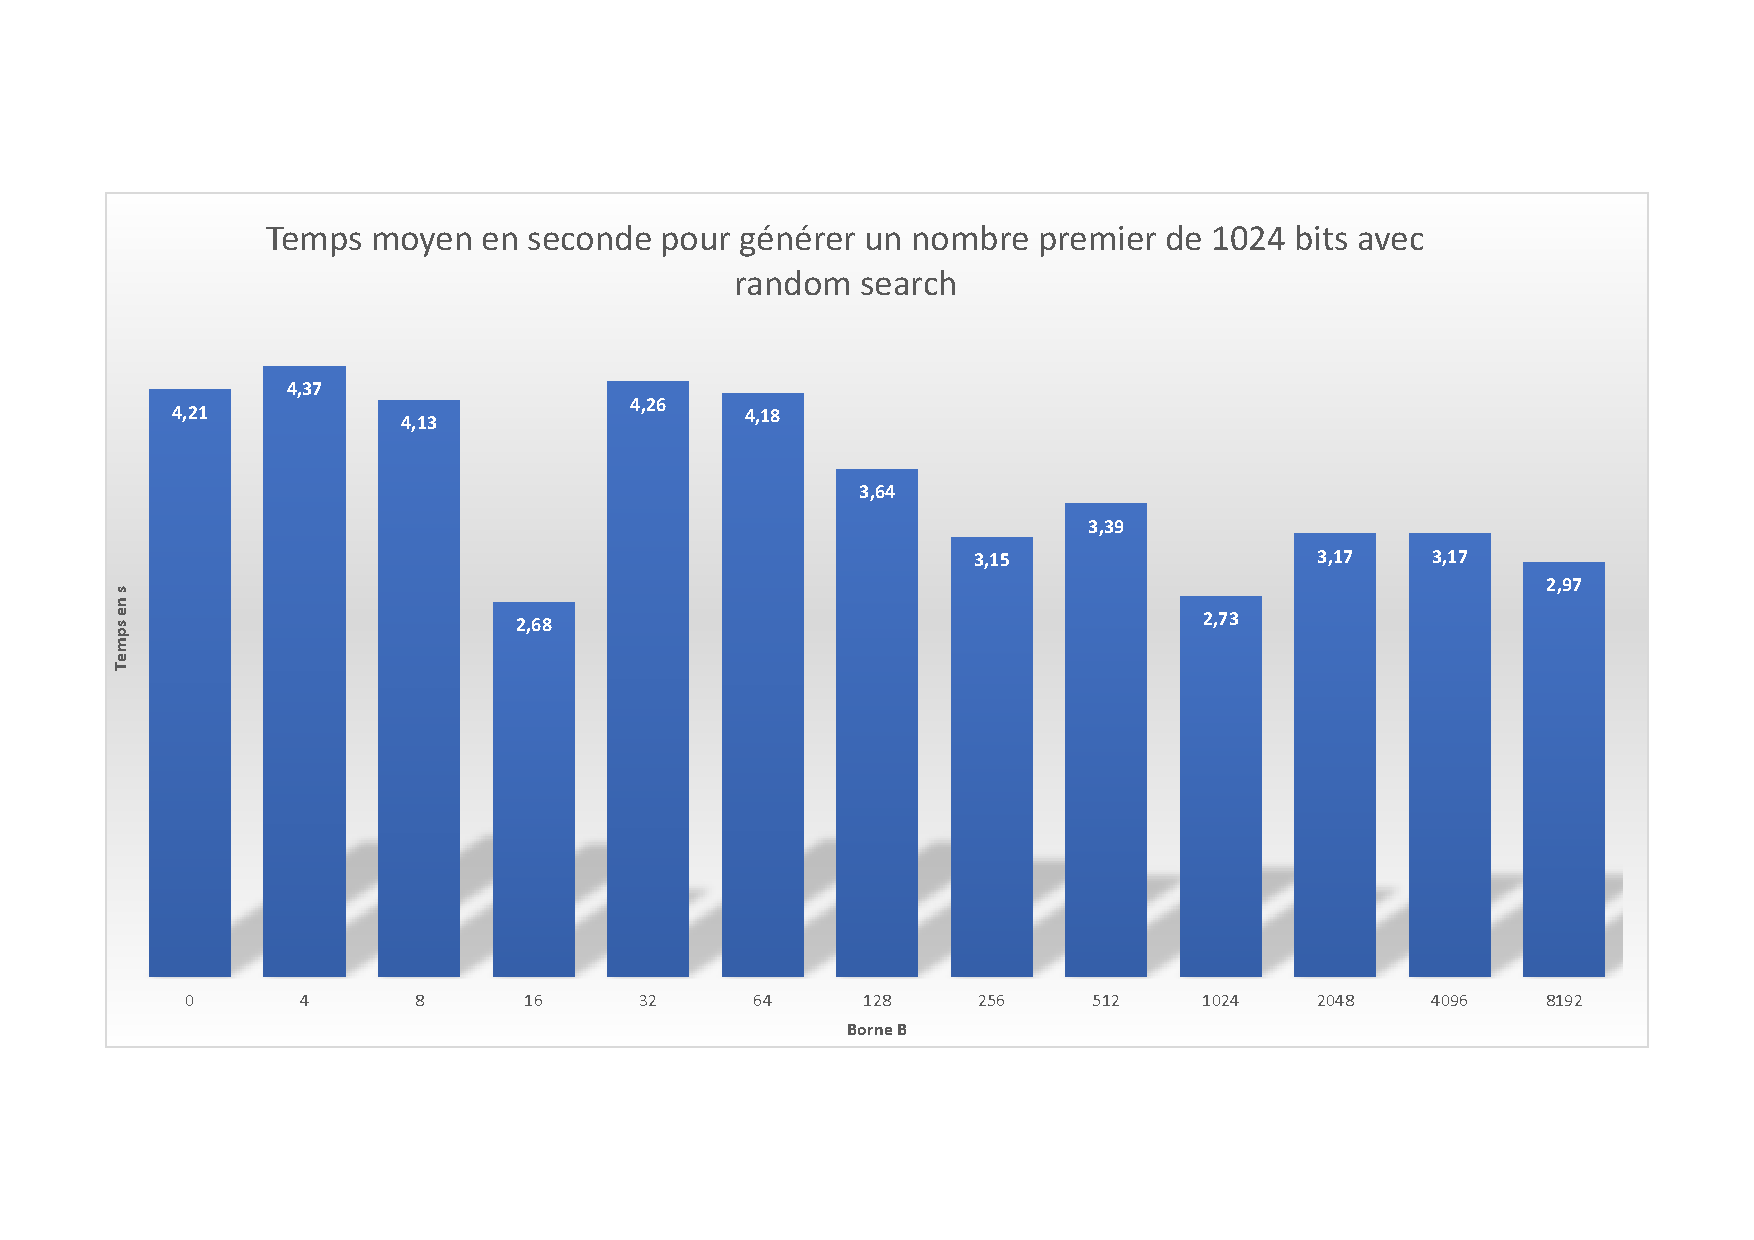
\includegraphics[scale=0.6]{Figures/Graphique.pdf}
    \caption{Graphique moyenne en seconde sur $100$ tests. }
\end{figure}

Voici un graphique récapitulant les tests menés pour générer un nombre premier de $1024$ bits avec RandomSearch et diffèrente valeur de B.
Il semblerait que la valeur optimale pour B spécifique à notre implémentation soit B=16. 

\subsubsection{Choix du paramètre de sécurité t}

Voici le tableau récapitulant les valeurs de $t$ en fonction de la taille du nombre premier a générer pour satisfaire la sécurité décrite \ref{Test probabiliste de primalité}. Ces résultat sont tirés du livre \cite{HAC}.

\begin{figure}[H]
    \centering
    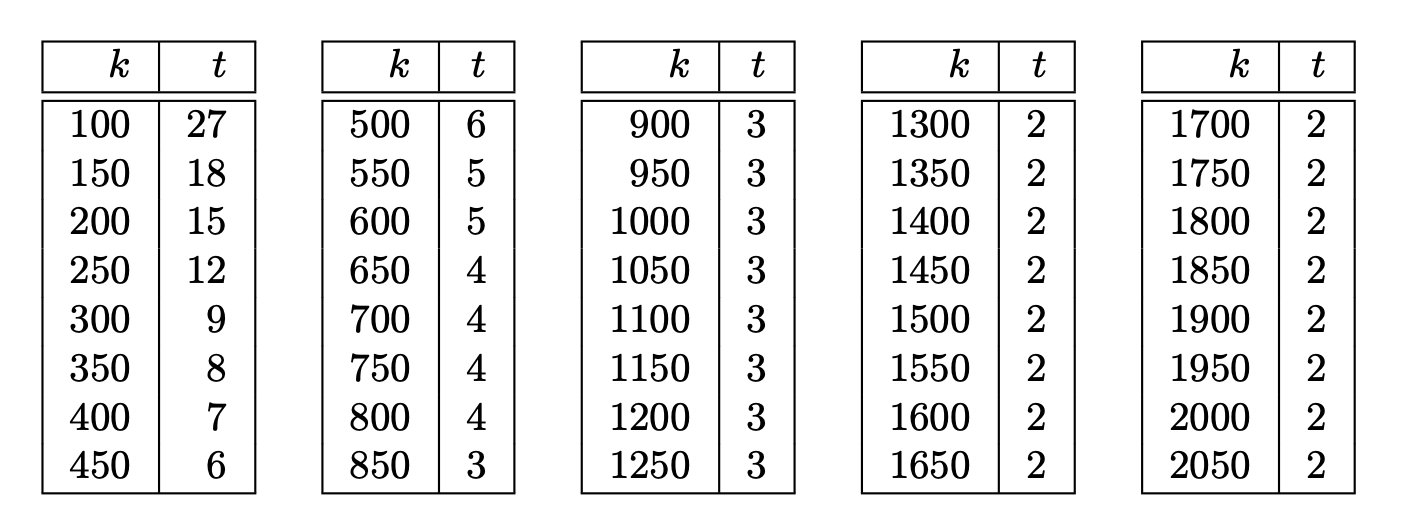
\includegraphics[scale=0.6]{Figures/parametret.png}
    \caption{Tableau des choix de $t$ en fonction de la taille du nombre premier a générer garantissant la sécurité demandée.}
\end{figure}

\section{Algorithme de Gordon}
\label{Algorithme de Gordon}
Le cryptosystème RSA utilise un nombre $n = pq$, où $p$ et $q$ sont des nombres premiers impairs. Les nombres premiers $p$ et $q$ doivent être d’une taille suffisante pour que la factorisation de leur produit soit hors de portée informatique donc d'une recherche exhaustive. La découverte du système cryptographique RSA a conduit à l’étude de contraintes sur le choix de $p$ et $q$ qui est nécessaire pour assurer que le système RSA soit à l’abri des attaques, ainsi la notion d’un premier fort a été définie. Actuellement la meilleure attaque connue est de l'ordre de 712 bits pour casser le système. De nos jours, la notion de nombre premier fort n'est pas forcément utilisé dans tous les systèmes car générer des nombres de 2048 bits est hors de portée d'attaque. Enfin, un nombre premier de 2048 bits peut-être généré par RandomSearch ou Gordon et il faut savoir qu'une clé n'est pas générer tous les jours elle est utilisée assez longtemps. Définissons quand même la notion de nombre premier fort pour la suite et l'utilisation de l'algorithme de Gordon.
\subsection{Nombre premier fort}

Les \textbf{nombres premiers forts} sont utilisés pour générer les clés de codage en cryptographie RSA. Ces nombres créent des cas de résolution impossibles pour ceux qui chercheraient à factoriser les clés du code.

\underline{\textbf{Définition:}}

Un nombre premier est dit \textbf{nombre premier fort} si les entiers r,s et t existent et si les conditions suivantes sont satisfaites:

\begin{enumerate}[label=\arabic*)]
 \item   $ p-1$ à un grand facteur premier noté $r$
 \item   $ p+1$ à un grand facteur premier noté $s$
 \item  $r-1$ à un grand facteur premier noté $t$
\end{enumerate}


Si on prend un exemple, $71$ est un nombre premier fort car il satisfait les conditions ci-dessus. En effet $p=71$, $71=7*10+1$ de plus $7=2*3+1$ et $71=36*2-1$. 

Un nombre premier fort générer pour RSA doit être beaucoup plus grand que cet exemple. Par exemple des nombres de 1024 ou 2048 bits.

\subsection{Algorithme de Gordon et complexité}

Voici l'algorithme de Gordon qui permet de générer un nombre premier fort.

\begin{algorithm}
\caption{Gordon(nbits,$k=20$,$i_0=1$, $j_0=1$)}
\begin{algorithmic}[1]
\Require{Un entier nbits qui définit le nombre de bits }
\Ensure{un entier $p$ de nbits-bit}
\State \textbf{Générer} 2 grand nombres premiers $s$ et $t$ avec $RandomSearch(nbits,k)$
\State  \textbf{Choisir} un entier $i_0$. \textbf{Trouver} le premier nombre premier dans la séquence $2it+1$ pour $i=i_0,i_0+1,i_0=2,...$. \textbf{Noter} ce nombre premier $r=2it+1$
\State \textbf{Calculer} $p_0=2(s^{r-2} \mod r)s -1$
\State  \textbf{Choisir} un entier $j_0$. \textbf{Trouver} le premier nombre premier dans la séquence $p_0+2jrs$ pour $j=j_0,j_0+1,j_0+2,...$. \textbf{Noter} ce nombre premier $p=p_0+2jrs$.
\State \Return p
\end{algorithmic}
\end{algorithm}

Pour générer les 2 grands nombres premiers au début de l'algorithme, nous utiliserons l'algorithme de $RandomSearch(k,t)$. De plus, pour trouver le nombre premier $r$ et $p$ dans la séquence définit dans l'algorithme, on peut notamment utiliser le test de $MillerRabin(n,t)$ ou le test de $Pocklington$ notamment à l'étape 2 pour optimiser le temps de calcul.

\underline{\textbf{Complexité}}:

En utilisant le test de Miller-Rabin, le temps attendus par l'algorithme de Gordon pour trouver un nombre premier fort est d'environ $19\%$ plus grand que la complexité en temps trouvée par l'algorithme pour générer des nombres premiers aléatoires.

\subsubsection{Résultats Expérimentaux}

Nous avons codé notre algorithme avec $MillerRabin(n,t)$ pour tester les nombres $r$ et $p$ afin d'avoir un temps d'exécution proche de $RandomSearch(k,t)$. Nous n'avons pas pu finir pour coder l'algorithme avec le test de Pocklington à l'étape 2 car il est certain que ceci optimiserait le temps. 
On a pris un paramètre de sécurité $k=20$ comme cela on peut faire marcher l'algorithme facilement. Si on teste avec 1024 bits, l'algorithme nous retourne un nombre premier fort en environ 8 secondes ce qui n'est pas négligeable sachant toutes les propriétés à vérifier pour nombre premier fort.
Il est quand même plus logique d'utiliser l'algorithme $RandomSearch(k,t)$ qui comme on l'a dit dans l'introduction est plus efficace que l'algorithme de Gordon pour générer un nombre de 2048 bits premiers et nous garantit déjà d'une sécurité maximale.


\section{Algorithme DSA}
\label{Algorithme DSA}
\underline{\textbf{Définition}}:

 Parmi les nombres premiers forts qui sont utilisés pour générer des clés de codage, on trouve aussi les nombres \textbf{DSA} (Nist Digital Signature Algorithm) qui ont la même utilité. Ils ont plusieurs conditions spécifiques. L'algorithme DSA a besoin de deux nombres premiers $p$ et $q$ qui satisfassent les conditions suivantes:


\begin{enumerate}[label=\roman*)]
 \item  Soit un entier $q$ premier de 256 bits tel que,  $2^{255} \leq q \leq 2^{256}$. 
 \item   Soit un entier $p$ premier tel que ,  $2^{L-1} \leq p \leq 2^{L}$ avec $L=2048+64l$ pour $0\leq l \leq 8$,
 \item  $q$ divise $p-1$
\end{enumerate}

Cette algorithme présente donc comment construire les nombres p et q à partir d'une fonction de hachage. La fonction de hachage utilisé est la fonction Sha-2 qui produit des hachés de $256$ bits. 

Sha-2 est une fonction de hachage cryptographique conçue par la \textit{ National Security Agency} des Etats-Unis qui est un standard de traitement de l'information. Elle produit un résultat de 256 bits (32 octets), habituellement représenté par un nombre hexadécimal. Les algorithmes de la famille SHA-2 sont très semblables, il y a essentiellement deux fonctions différentes, SHA-256(utilisé dans l'algorithme) et SHA-512, les autres étant des variantes de l'une ou l'autre. Les fonctions SHA-256 et SHA-512 ont la même structure mais diffèrent par la taille des mots et des blocs utilisés. Cette structure est assez proche de celle de SHA-1, mais un peu plus complexe et en évite certaines faiblesses connues.

Ici, dans l'algorithme la fonction de Hachage sert notamment à produire les nombres premiers $q$ et $p$ grâce aux entiers $s$ et $s+1 \mod 2^g$. Tout d'abord, on convertit $H(s)$ et $H(s+1 \mod 2^g)$ en base 2 et ensuite on fait le "XOR" sur les entiers c'est-à-dire on fait une addition binaire des deux chaînes. Ensuite, pour trouver $q$ on remplace par 1 les bits de poids faible et de poids fort du résultat du XOR. Finalement, le test de primalité de Miller-Rabin assure le fait que $q$ est premier. Pour trouver $p$ on calcule W tel que: 

$W=V_0 + V_1*2^{256} + V_2*2^{512} +...+V_{n-1}*2^{256(n-1)} + (V_n\mod 2^b)2^{256n}$ avec $V_k=H(s+k+j \mod 2^g)$. 

Ensuite, on calcule un entier X de L bits tel que $X=W+2^{L-1}$. Enfin, on calcule $c=X\mod2^q$ et on définit $p=X-(c-1)$. Pour déterminer si $p$ est premier, on calcule la primalité de $p$ en utilisant le test de Miller-Rabin.
L'algorithme DSA renvoie donc les entiers premiers \textbf{p} et \textbf{q}.

\subsection{Algorithme NIST pour générer les nombres premiers DSA}

\begin{algorithm}[h!]
\caption{DSA(l)}
\begin{algorithmic}[1]
\Require{Un entier l, $0\leq l \leq 8$ }
\Ensure{$q$ un entier de 256 bits premier et p un premier de L bits tel que $L=2048+64l$ et $q|p-1$}
\State Calculer $L=2048+64l$ et trouver le reste $(b)$ et le quotient $(n)$ de la division de $L-1$ par 256   
\State \textbf{Répéter les actions suivantes:}
\State Trouver un entier $s$ aléatoire de longueur binaire $ \leq 256$
\State Calculer $U=H(s) \oplus H(s+1 \mod 2^g)$ et former $q$ grâce à $U$ en remplaçant par 1 le bits de poids faible et de poids fort.
\State Calculer MillerRabin($q$,$t$) pour $t\geq18$ jusqu'à que $q$ soit premier sinon on recommence les étapes.
\State Soit $i=0$ et $j=2$
\While { $i < 4096$ }
\For {$k$ \textbf{allant de} 0 \textbf{à} $n$}
\State $V_k=H(s+k+j \mod 2^g)$ 
\State $W=V_0 + V_1*2^{256} + V_2*2^{512} +...+V_{n-1}*2^{256(n-1)} + (V_n\mod 2^b)2^{256n}$ 
\EndFor
\State $X=W+2^{L-1}$
\State Calculer $c=X\mod2^q$ et définir $p=X-(c-1)$
\If{$p\geq2^{L-1}$ }
\State Utiliser MillerRabin($p$,$t$) pour $t\geq5$. 
\State Si p est premier probable alors \Return (p,q)
\EndIf
\State définir $i=i+1$ et $j=j+n+1$
\EndWhile
\State Revenir à l'étape 2
\end{algorithmic}
\end{algorithm}

\subsubsection{Résultats Expérimentaux}

A la base, l'algorithme est présenté avec la fonction de Hachage Sha-1. C'est fonction n'est plus considéré comme sûr contre des adversaires disposant de moyens importants. En 2005, des cryptanalystes ont découvert des attaques sur SHA-1, suggérant que l'algorithme pourrait ne plus être suffisamment sûr pour continuer à l'utiliser dans le futur. En 2010, Sha-1 a été remplacé par la fonction que nous avons décidé d'utiliser: Sha-2.

Prenons par exemple en entrée un entier l=1. L'algorithme $DSA$ renvoie les entiers $p$ de 2048 bits et $q$ de 256 bits en moyenne en 5 secondes. 

\clearpage

\section{Génération de nombre premiers de Sophie Germain}

\underline{\textbf{Définition}}:

Un nombre premier $p$ est appelé \textbf{nombre premier de Sophie Germain} si $2p+1$ est aussi un nombre premier.
Le nombre $2p + 1$, associé à un premier de Sophie Germain est un \textbf{nombre premier sûr} (safe prime).

Exemple: $11$ et $2*11+1 = 23$ sont tous deux premiers.

Une séquence (chaîne de Cunningham)  apparaît lorsque le nombre associé est lui-même un nombre premier de Sophie Germain. Exemple de séquence à cinq termes:

2, 2x2+1 = 5, 2x5+1 = 11, 2x11+1 = 23, 2x23+1 = 47

\underline{\textbf{Remarque}}:

Finalement, en pratique, pour tester si un nombre est de Sophie Germain il faut appliquer la méthode suivante :

Soit $p$ un nombre premier de la forme $p=4k+3$. Alors $p$ est un nombre premier de Sophie Germain si et seulement si le nombre de Mersenne $M_p = 2^{p} - 1$ est un nombre composé dont $2p+1$ est un diviseur. Cette proposition peut être utilisée comme test de primalité et c'est comme cela que l'on peut faire des records de nombres premiers de Sophie Germain.


\subsection{Historique}

Sophie Germain (1776-1831) est une des premières femmes mathématiciennes. Brillante autodidacte, estimée par quelques uns de ses pairs, elle s'est toutefois heurtée à l'intransigeance de son époque envers les femmes savantes.
A 19 ans, elle parvient à obtenir les notes de cours de l'Ecole Polytechnique nouvellement créée. Pour pouvoir se consacrer aux mathématiques, alors réservées aux hommes, elle utilisa un nom d’emprunt de 1794 à 1807 : Antoine Auguste Le Blanc. Elle commence à entretenir une correspondance avec Lagrange, qui y est professeur d'Analyse.

La théorie des nombres est le premier domaine où Sophie Germain apporte une contribution importante. On lui doit notamment les plus importantes avancées sur le théorème de Fermat depuis Euler (1738), et avant Kummer (1840). Elle démontre que si n est un nombre premier (distinct de 2) tel que $2n+1$ est un nombre premier, alors un triplet d'entiers (x,y,z) ne peut vérifier l'équation de Fermat :
\begin{center}
$x^n + y^n = z^n$.
\end{center}
Elle décrit aussi une classe particulière de nombres, devenus les nombres premiers de Sophie Germain. Un nombre est de ce type si son double plus 1 est premier aussi.

A la suite de la visite du physicien allemand Chladni à Paris en 1809, Sophie Germain change radicalement d'orientation mathématique. Pendant plus d'une décennie, elle s'intéressera à la théorie des surfaces (principalement à leur courbure) et au problème de vibration des surfaces élastiques. Sophie Germain continue à travailler jusqu'à la fin de sa vie sur les mathématiques et la philosophie. Elle décède le 27 juin 1831, victime d'un cancer du sein.




\printbibliography
\cite{HAC}
\cite{frwiki:Primalité}
\cite{frwiki:Sophie_Germain}
\cite{Preuve_Miller-Rabin}
\addcontentsline{toc}{chapter}{Bibiliographie}

\newpage
\thispagestyle{empty}
\addcontentsline{toc}{chapter}{Implémentation}
\mbox{}
\newpage












\end{document}
\pagenumbering{arabic}

